\section{How to Verify JML Specifications with the \kt}
\label{sec:analyze}

JML specifications, in particular pre-~and postconditions, can be seen
as abstractions of an implementation.  In this context, an
implementation is called {\em correct} if it actually implies the
properties expressed in its specification. The \kt\ includes
functionality to {\em verify} the correctness of an implementation
with respect to its specification. 

In this section, we describe how to start (Sect.~\ref{sec:starting})
the \kp\ and load the tutorial example (Sect.~\ref{sec:loading}) as
well as a short overview about the graphical user interface and its
options (Sect.~\ref{sec:prover}). Last but not least, we explain
how to configure the \kp\ to follow the tutorial example
(Sect.~\ref{sec:configure}).


\subsection{Starting the \kp}
\label{sec:starting}

In order to verify a program, you first need to start the \KeY\
prover. This is done either by using the webstart mechanism (see
Sect.~\ref{install:javaws}) or by running the jar file from 
your \KeY\ distribution\footnote{In
  this case we assume that you have installed the \kt\ as described in
Sect.~\ref{install:byteandsourcecode}.}, e.g.,~by
running
  \begin{center}
    \texttt{java -jar key.jar} 
  \end{center}

% Eclipse is atm unsupported
%\noindent If you use the Eclipse intall, start the \kp\ as stand-alone tool via
%the menu \mea{Verification}. 

\subsection{Loading the Tutorial Example}
\label{sec:loading}

After downloading and unpacking this quicktour, you should find a
directory containing the two subdirectories
\texttt{paycard} and \texttt{gui}. We refer to the directory
\texttt{jml} as top-level directory.


\begin{enumerate}
\item You have to choose the Java source files you want to
  verify. They contain both the source code and the JML
  annotations. You can do this by either
\begin{itemize}
  \item adding the path to the \texttt{paycard}
    directory to the command:
    \begin{center}
      \texttt{java -jar key.jar <path\char`\_to\char`\_quicktour>/jml/paycard}  
    \end{center}
  \item opening \meb{File}{Load} and selecting the \texttt{paycard}
    package directory after having started \KeY\ without
    any arguments.
\end{itemize}

\KeY\ will then load the tutorial example and parse the JML
annotations. If you get an error dialog similar to the one in
  Fig.~\ref{fig:error:unknownType}, you have selected the
  \texttt{jml} directory instead of its subdirectory \texttt{paycard}.

\begin{figure}
\centering
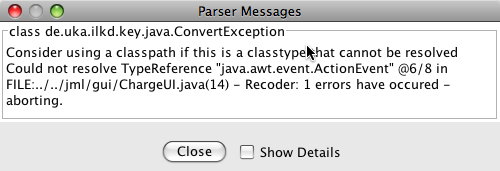
\includegraphics[width=0.75\textwidth]{../figures/errorDialogUnknownType}
\caption{Error dialog complaining about an unknown type}
\label{fig:error:unknownType}
\end{figure}

If you have your own projects you want to verify, you can proceed
similarly. Please note that \KeY\ by default supports only a very
limited selection of the standard library classes.
How to extend them and how to
configure more complex projects that use 3rd party libraries is
described in brief in App.~\ref{app:configuringProjects}.

\item Now the \prm{} window should appear as shown in
  Fig.~\ref{fig:pob:startup}.
  
  \begin{figure}[hp]
    \centering
    \subfigure[\pob\ after startup with expanded \jn{paycard}
    package\label{fig:pob:startup}]{ \centering
      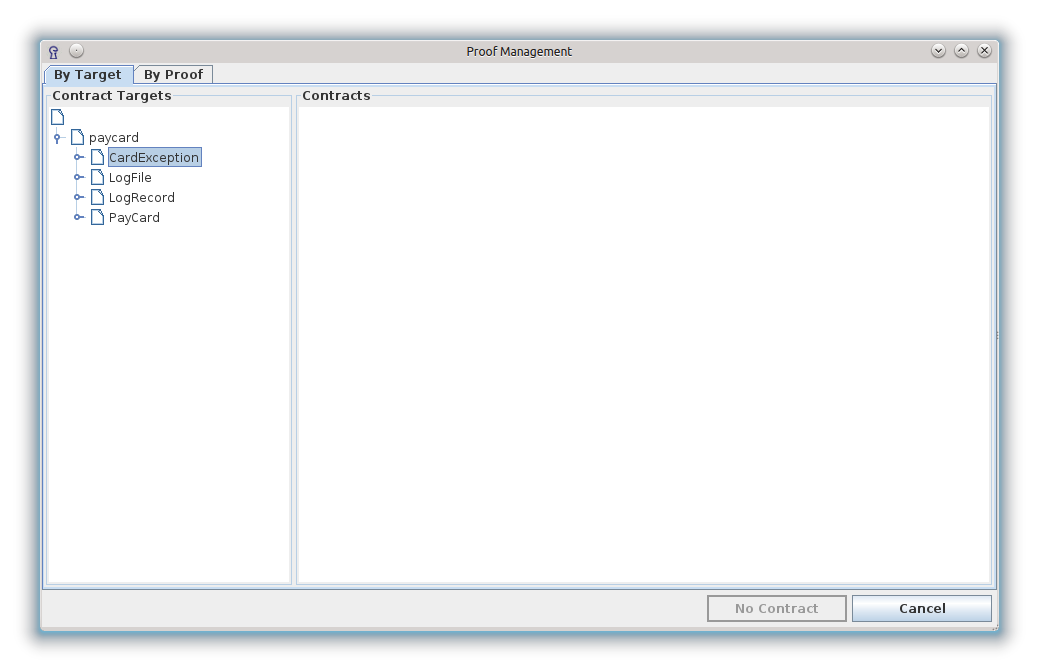
\includegraphics[width=\textwidth]{../figures/proofmanagement}
    }
    \subfigure[\pob\ listing proof obligations for \jn{PayCard::charge} \label{fig:pob:expandedProofObligations}]{
      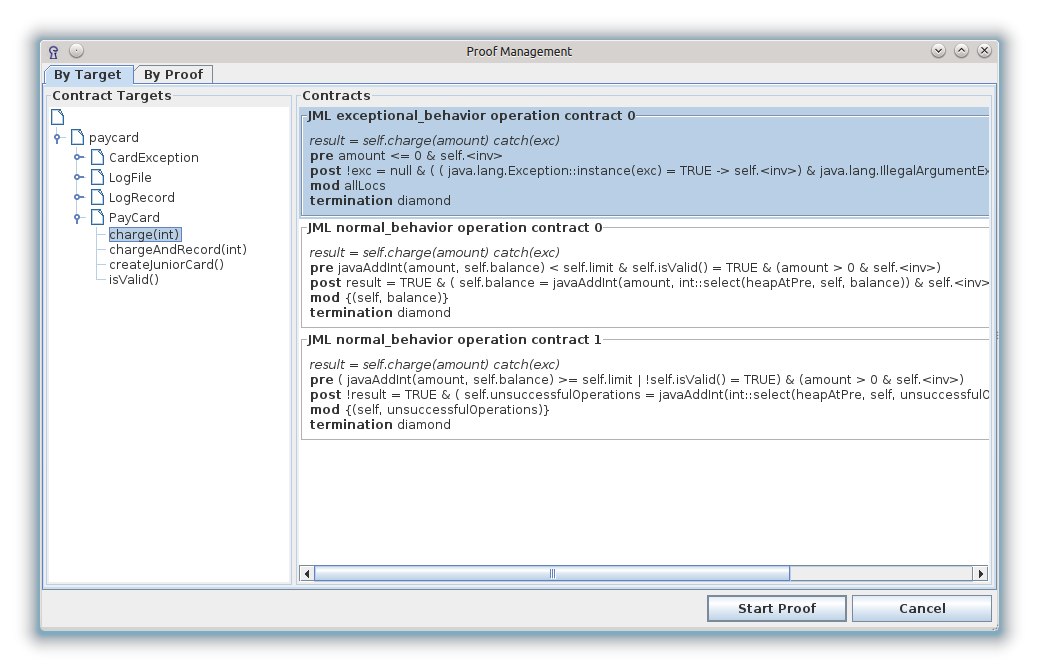
\includegraphics[width=\textwidth]{../figures/proofmanagement_paycard}
    }
    \caption{The \pob\ window}
    \label{fig:proofObligationBrowser}
  \end{figure}

  In the left part of the window titled \mea{Contract Targets},
  the \prm{} lists all packages, classes, interfaces, and methods of the
  project to be verified in a tree structure similar to standard file
  managers.

  The browser allows you to select the proof obligation you want to verify. 
  Selecting \jn{PayCard::charge} gives you three contracts
  (Fig.~\ref{fig:pob:expandedProofObligations}):
  one \mea{exceptional\_behavior}
  and two \mea{normal\_behavior} contracts. Select the first \mea{normal\_behavior}
  contract
  and confirm by pressing the button \mea{OK}. More details about the
  contract configurator will be given in Sect.~\ref{sec:provableProp}.

\item You should now see the \kp\ window with the loaded proof
  obligation as in Fig.~\ref{fig:proverWithLoadedPO}. The prover is
  able to handle predicate logic as well as dynamic logic. The \kp\
  was developed as a part of the \KeY project and is implemented in
  \textsc{Java}. It features interactive application of proof rules
  as well as automatic application controlled by strategies. In the
  near future more powerful strategies will be available.

  In Sect.~\ref{sec:application}, we show how to prove some of the
  proof obligations generated for the tutorial example.
\end{enumerate}

  \begin{figure}
    \centering
    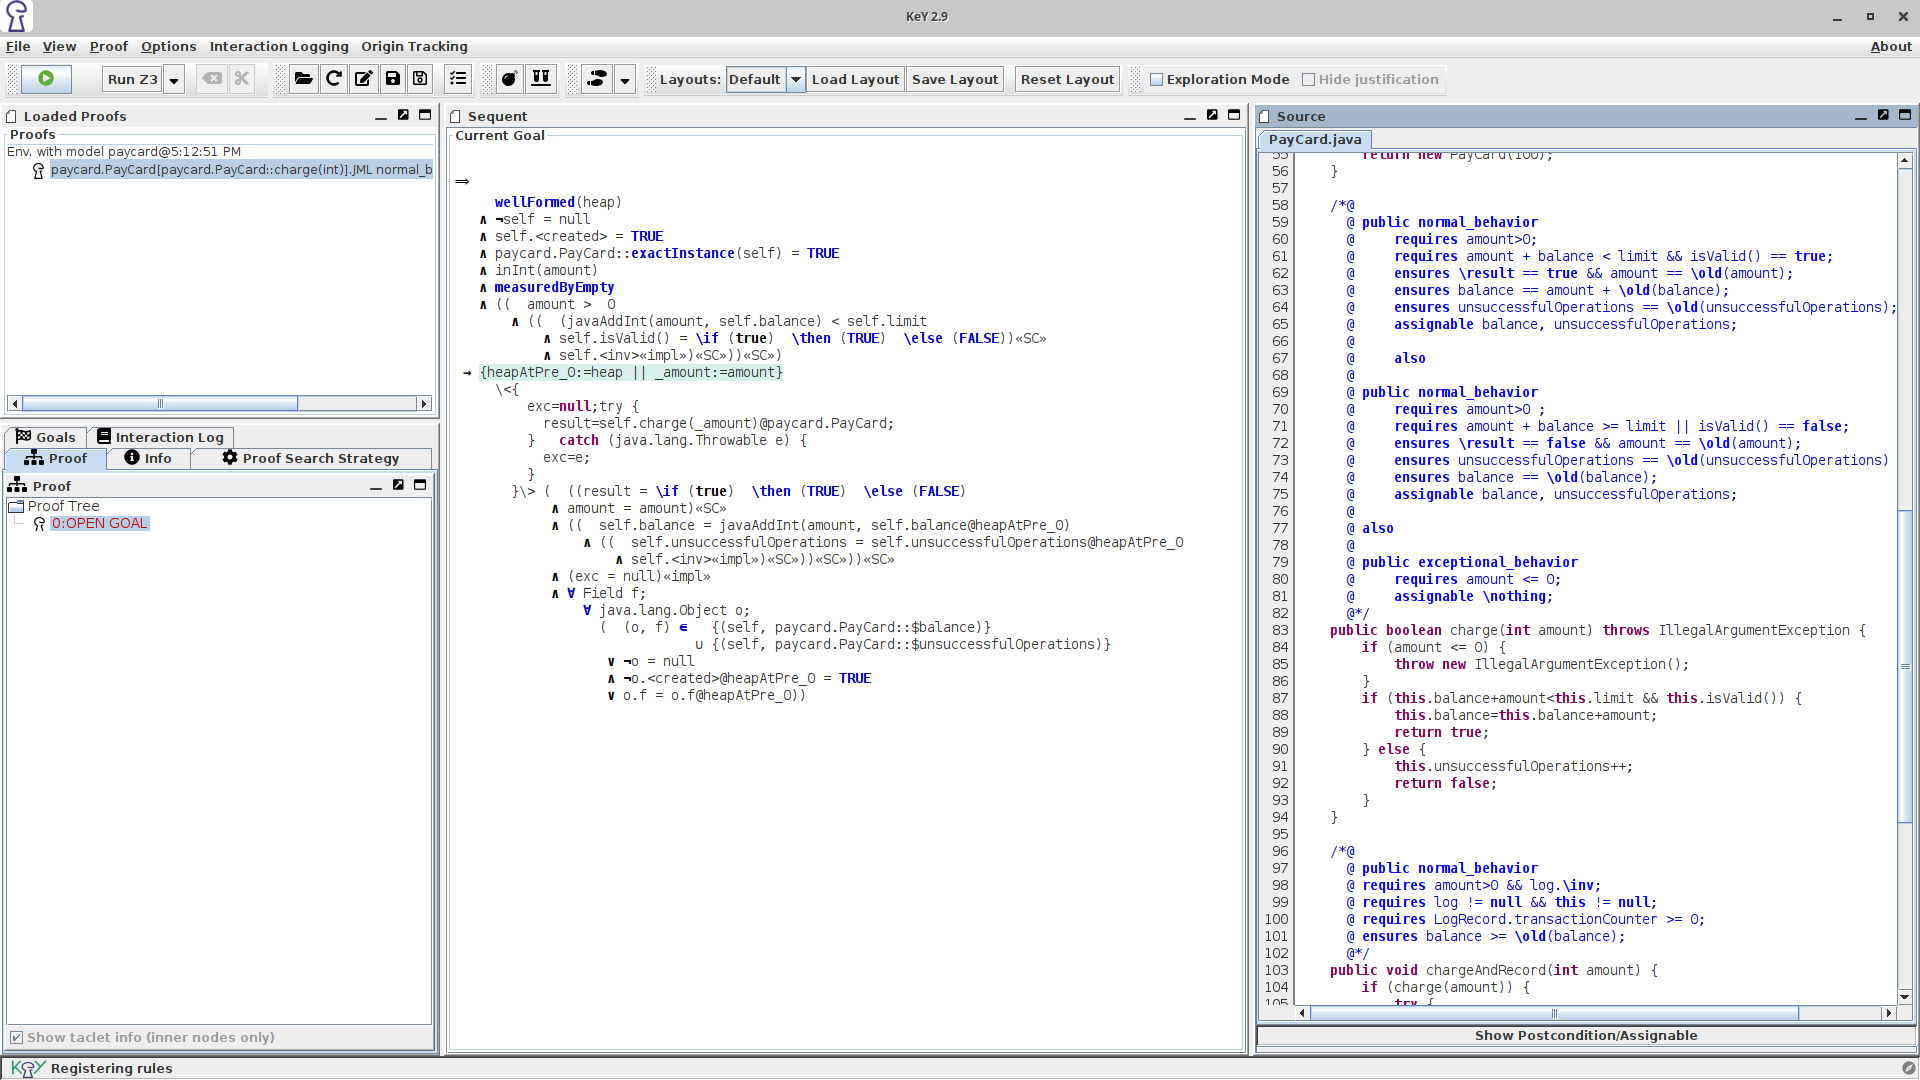
\includegraphics[width=\textwidth]{../figures/proverWithLoadedPO}
    \caption{The \kp\ with the contract
      for \jn{charge} loaded.}
    \label{fig:proverWithLoadedPO}
  \end{figure}


\subsection{The \kp} 
\label{sec:prover}

We assume that you have performed the steps described in the previous
section and that you see now something similar to
Fig.~\ref{fig:proverWithLoadedPO}. In this section, we describe the GUI
of the \kt\ and its different components. Most of the components in
the GUI are also labeled with a tooltip.


The \kp\ window consists of a menubar, a toolbar (all buttons explained in~\ref{app:shortcuts}) 
and three panes where 
the lower left pane is additionally tabbed. Each pane is described below.
%
The layout of the three panes can be changed by the user. Layouts can be saved and loaded
in the \meb{View}{Layout} menu.

\begin{description}

\item[Upper left pane:] Every problem you want to prove with the \kp\
is loaded in a proof environment. In this pane, all currently loaded
problems respectively their proof environments are
listed.


\item[Lower left pane:] This pane contains the following five tabs.
  
  \begin{description}
  \item[Proof:] This pane (see Fig.~\ref{fig:prover:tab:proof})
      contains the whole proof tree which represents the current
      proof. The nodes of the tree correspond to sequents (goals) at
      different proof stages. Click on a node to see the corresponding
      sequent and the rule that was applied on it in the following
      proof step (except if the node is a leaf). Leaf nodes of an open
      proof branch are colored red whereas leaves of closed branches
      are colored green.
    
      Pressing the right mouse button on a node of the proof tree will
      open a pop-up context menu. If you choose \tn{Prune Proof},
      the proof tree will be cut off at this node and all nodes lying
      below will be deleted. Choosing \tn{Apply Strategy} will start
      an automatic proof search (see later \tn{Automatic Proving}),
      but only on the branch which the node you had clicked on belongs to.
      
      The context menu also contains commands that allow you to hide
      closed subtrees, to hide inner nodes, to collapse, or to expand
      the tree. The commands help you to keep track of a large proof.
    
  \item[Goals:] In this pane, the open goals of a certain proof
    (corresponding to one entry in the upper left pane) are listed. To
    work on a certain goal just click on it and the selected sequent
    will be shown in the right pane.
    
%   \item[User Constraint:] To explain this functionality would go
%     beyond the scope of this quicktour. It won't be required in the
%     sequel.

  \item[Info:] In this pane (Fig.~\ref{fig:prover:tab:rules}), all the
    rules, term labels, and function symbols
    available in the system are indicated.
    
    For the rules, \KeY\ distinguishes
    between \tn{axiomatic taclets} (rules that are always true in the
    given logic), \tn{lemmas} (that are derived from and thus provable
    by axiomatic taclets) and \tn{built-in rules} (for example how
    certain expressions can be simplified).
    
    By clicking on a rule of the list, the description of that rule is
    shown in the box below the rule list.
    
    Term labels are additional information that can be attached to a term.
    They do not change a term's semantics, but are used to guide the poof
    search or to carry non-logical information about a term, like its
    corresponding line number in the source code.
    
    The function symbols folder lists all interpreted function and predicate
    symbols in the dynamic logic.
    
  \item[Proof Search Strategy:] This tab (see
    Fig.~\ref{fig:prover:tab:strategy}) allows you to define the active
    strategy from a set of available strategies. There are several
    parameters and only the most important ones will be covered here, 
    a complete list can be found in~\ref{app:strategy}:

    \begin{description}
%     \item[Autoresume strategy] By checking this you tell KeY to continue automated proof search after user interaction.

    \item[Max. Rule Applications] You can set the number $N_{aut}$ of
      automatic rule applications using the slider. Even if the
      automatic strategy can still apply rules after $N_{aut}$
      applications, automatic proving stops. 


    \item[Stop At] Choose when strategy execution shall stop.
      Possible values are \texttt{Default}: strategy stops when no
      rules are applicable or the maximal number of steps is reached and
      \texttt{Unclosable}: strategy stops in all situations when
      \texttt{Default} stops but also already when the first goal is
      encountered on which no further rule is (automatically) applicable. 

    \item[Proof splitting] Influences usage of rules branching a
      proof tree. Only rules working on formulas not on
      programs fall under the chosen policy, i.e., program rules
      causing
      splits are still applied even if splitting is switched off. The
      values are \texttt{free} (withour restrictions), \texttt{Delayed}
      (allows still splitting but prefers other rules) and \texttt{Off} (no
      splitting).

    \item[Loop treatment] This setting determines how while-loops are
      treated. They can be left untouched (\texttt{None}), handled
      using stated invariant contracts, or
      repeatedly unrolled (\texttt{Expand}). If handled using invariants,
      you can either choose the new \texttt{Loop Scope} rule (recommended),
      or the legacy \texttt{Transformation}-based rule.

    
    \item[Method treatment] Methods can also be left untouched
      (\texttt{None}), have their method contracts applied
      (\texttt{Contracts}), or be inlined, i.e. have the method body
      expanded in place (\texttt{Expand}).
      
    \item[Dependency contract] For the simplification of heap terms, setting this option to \texttt{On}
				the information in JML's \texttt{accessible} clause is used. 

   \item[Arithmetic treatment] The \kp\ has several options for the treatment of arithmetic expressions:
   \begin{description}
   \item[Basic:] Using this option, polynomial expressions are simplified. 
		 In the antecedent Gr\"{o}bner Bases are computed polynomials.
		 Linear inequations are handled using (partial) Omega procedures.

   \item[DefOps:] Using the option \textsf{DefOps}, mathematical symbols such as:\\
                \texttt{/}, \texttt{\%}, \texttt{jdiv}, \texttt{jmod}, range predicates, such as
                \texttt{int\_RANGE}, \texttt{short\_MIN} and symbols for mathematical operations on 
                integers with a certain semantic such as
                \texttt{addJint} or \texttt{mulJshort}, are expanded. This means for example constants, 
                such as \texttt{short\_MIN}, are  
		 replaced by their concrete values (in this case -32768) and range predicates, 
		 such as \texttt{inInt} are replaced by their ranges 
		 (in this case $i \leq int\_MAX \wedge int\_MIN \leq i$).
		 
                
    \item[Model Search:] Setting the \textsf{model search} option, 
		  the \kp\ supports non-linear equations and model search.
		  Additionally multiplication of inequations with each other
		  and systematic case distinctions  (cuts) can be performed.
                This method is guaranteed to find counterexamples for
                invalid goals that only contain polynomial (in)equations.
                Such counterexamples turn up as trivially unprovable goals.
                It is also able to prove many more valid goals involving
                (in)equations, but will in general not terminate on such goals.
                
   \end{description}
   
   \item[Quantifier treatment] Sometimes quantifiers within the
      sequent have to be instantiated. This can be either done
      manually (\texttt{None}) or automatically with different
      alternatives:
      \begin{description}
        \item[No Splits] Instantiate a quantifier only if
          this will not cause the proof to split.
        \item[Unrestricted] Instantiates a quantifier even
          when causing splits. However the startegy tries to predict
          the number of caused open branches and will prefer those
          with no or only few splits.
        \item[No Splits with Progs] Chooses between the
          \texttt{No Splits} and \texttt{Unrestricted} behaviour
          depending on programs present in the sequent. If a program is
          still present the \texttt{No splits} behaviour is
          used. Otherwise quantifiers are instantiated unrestricted
      \end{description}
    \end{description}   
  \end{description}

\item[Middle pane:] In this pane, you can either inspect inner, already
  processed, nodes of the proof tree or you can continue the proof by
  applying rules to the open goals, whichever you choose in the left
  pane.

  Rules can be applied either interactively or non-interactively
  using strategies:

  \begin{description}
  \item[Interactive Proving:]
    By moving the mouse over the current goal you will notice that a
    subterm of the goal is highlighted (henceforth called the
    \emph{focus term}). Pressing the left mouse button displays a list
    of all proof rules currently applicable to the focus term.
    
    A proof rule is applied to the focus term simply by selecting one of
    the applicable rules and pressing the left mouse button. The effect
    is that a new goal is generated. By pushing the button \tn{Goal
      Back} in the main window of the \kp\ it is possible to undo one or
    several rule applications. Note, that it is currently not possible
    to backtrack from an already closed goal.
    
  \item[Automatic Proving:] Automatic proof search is performed
    applying so-called strategies which can be seen as a collection of
    rules suited for a certain task. To determine which strategy
    should be used select the tab item \tn{Proof Search Strategy} in
    the left pane as described above.
     
    To start (respectively continue) the proof push
    the \tn{run strategy}-button on the toolbar labelled with the
    $\rhd$ - symbol.
    
%    Another way to define the strategy that should be used during the
%    current proof is to click on the field right to the \tn{run
%    strategy}-button. In this field the current strategy is
%    shown. After clicking on it, a list of all available strategies
%    comes up from which you can select one. By moving the blue arrow
%    to the left or to the right you can also set the maximum number of
%    automatic rule applications.

  \end{description}

\item[Right pane:] In this pane, you can see the Java source files pertaining
to the currently selected proof. When mousing over a term in the middle pane,
the corresponding JML specification in the right pane is highlighted in orange.
As you advance in the proof, the source code line corresponding to the current
proof state is highlighted in green.
\end{description}

\begin{figure}
  \centering
  \subfigure[The \textsf{Proof} tree tab\label{fig:prover:tab:proof}] {
    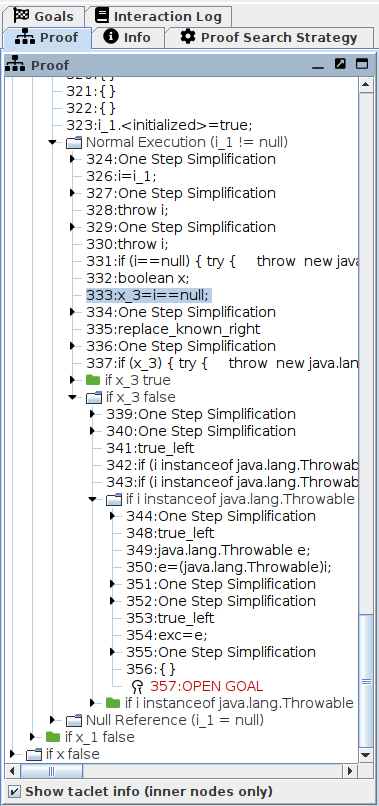
\includegraphics[width=0.357\textwidth]{../figures/proofTreeTab}
  }
    \subfigure[The \textsf{Info} tab\label{fig:prover:tab:rules}] {
    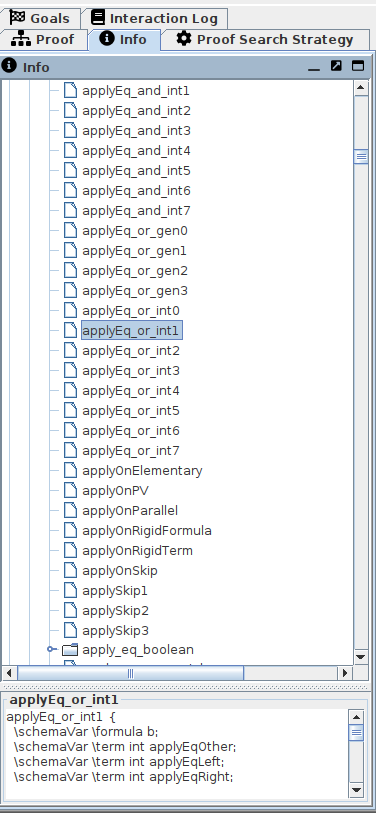
\includegraphics[width=0.35\textwidth]{../figures/infoTab}
  }  
  \subfigure[The \textsf{Proof Search Strategy} tab\label{fig:prover:tab:strategy}] {
    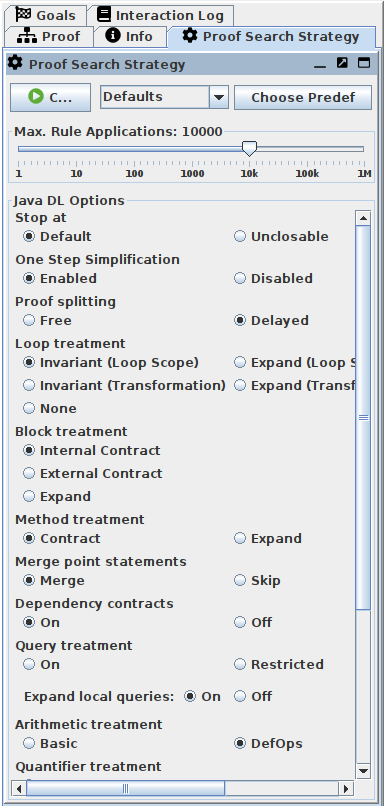
\includegraphics[width=0.35\textwidth]{../figures/strategyTab}
  }

  \caption{Selected components of the \kt\ graphical user interface}
  \label{fig:prover:components}
\end{figure}

\subsection{Configure the \kp}
\label{sec:configure}

In this section, we explain how to configure the \kp\ to follow the
tutorial and give a few explanations about the implications of the
chosen options. Most of the options are accessible via the \kp\
menu. An exhaustive list is available as part of
Appendix~\ref{app:menuOptions}. In order to verify or change some of
the necessary options, it is necessary to have a proof obligation
loaded into the \kp\ as described in Sect.~\ref{sec:loading}.

The menu bar consists of different pull-down menus:

\begin{description}
  \item[File] menu for file related actions like loading and saving
    of problems resp.\ proofs, or opening the \prm{} window
  \item[View] menu for changing the look of the \kp
  \item[Proof] menu for changing and viewing proof specific options
  \item[Options] menu for configuring general options affecting any proof
  \item[About] menu (as the name says)
\end{description}

\KeY\ provides a complete calculus for the Java Card 2.2.x version
including additional features like transactions. Further, it provides
some more concepts of real Java like class and object initialization.
This quicktour is meant to help with the first steps in the system.

For simplicity, we deactivate some advanced concepts and configure the \kp\ to
use the normal arithmetic integers to model Java integer types, which
avoids dealing with modulo arithmetics. \emph{Important:} Please
note that this configuration is unsound with respect to the Java
semantics.

In order to configure the \kp\ in this way, select
\meb{Options}{Show Taclet Options}. The dialog shows a list of
available options. 
Clicking on an option in the list also shows a short explanation
for the option.
The list below explains the options necessary for
this tutorial\footnote{App.~\ref{app:menuOptions} contains a list of
  all available options.}. Please ensure that for each option, the
value as given in parentheses directly after the option name is
selected. In case you have to change one or more values, you will have
to reload the tutorial example in order to activate them.

\begin{description}
      \item[JavaCard:] (\textsf{off}) There are two values for this option:
      \textsf{on} and \textsf{off}. Switches all
      taclets axiomatising JavaCard specific features like
      transaction on or off. 
  
   \item[initialisation:] (\textsf{disableStaticInitialisation})
      Specifies whether static initialization should be considered.

    \item[intRules:] \label{sec:integersem}
      (\textsf{arithmeticSemanticsIgnoringOF}) Here you can choose
      between different semantics for Java integer arithmetic (for
      details
      see~\cite{Schlager02,SchlagerPhD2007,KeYBook2007}). Three
      choices are offered:

      \begin{description}

      
      \item[\textsf{javaSemantics}] (Java semantics): Corresponds
        exactly to the semantics defined in the Java language
        specification. In particular this means, that arithmetical
        operations may cause over-/underflow. This setting provides
        correctness but allows over-/underflows causing unwanted
        side-effects.
      \item[\textsf{arithmeticSemanticsIgnoringOF}] (Arithmetic
        semantics ignoring overflow): Treats the primitive
        finite Java types as if they had the same semantics as
        mathematical integers with infinite range. Thus this setting
        does not fulfil the correctness criteria.
      \item[\textsf{arithmeticSemanticsCheckingOF}] (Arithmetic
        semantics prohibiting overflow): Same as above but the result
        of arithmetical operations is not allowed to exceed the range
        of the Java type as defined in the language
        specification. This setting not only enforces the java
        semantics but also ascertains that no overflow occur.
      \end{description}

\end{description}

\emph{Please} activate \tn{Minimize Interaction} in the
\texttt{Options} menu in order reduce interaction with the system.

As a last preparation step, change to the \textsf{Proof Search
  Strategy} tab in the lower left pane and choose the following setting:
\begin{itemize}

\item \textsf{Max. Rule Applications} should be set to a value greater
  or equal 500. A too low value will cause the prover to leave
  automatic mode too early. In that case, you might have to press the
  run strategy button more often than described in the tutorial.
\item \textsf{Java DL} must be selected with the following sub
  options:
  \begin{itemize}

    \item Stop at: \textsf{Default}
   \item Proof splitting: \textsf{Delayed} (\textsf{Normal} should
      also work)
    \item Loop treatment: \textsf{Invariant (Loop Scope)} 
    \item Method treatment: \textsf{Expand}
    \item Query treatment: \textsf{Expand}
    \item Expand Local Queries: \textsf{On}
    \item Arithmetic treatment: \textsf{Basic} is sufficient for this
      tutorial (when using division, modulo or similar you will need
      at least \textsf{DefOps})
    \item Quantifier treatment: \textsf{No Splits with Progs} is a
      reasonable choice for most of the time
    \item User-specific taclets: all \textsf{Off}
  \end{itemize}
\end{itemize}
 


%%% Local Variables: 
%%% mode: latex
%%% TeX-master: "quicktour"
%%% End: 
